% Directional collapse: evidence-backed ACL/ARR draft.
% Main-table and story revision 2026-10-10.
% Scientific numbers and tables are generated from audited campaigns.
% Build: make paper. See README.md and ARGUMENT.md.

\documentclass[11pt]{article}

% "review" = anonymous with line numbers, which is what ARR wants at submission.
% Switch to "final" for camera-ready, or "preprint" for a named version with page numbers.
\usepackage[review]{acl}

\usepackage{times}
\usepackage{latexsym}
\usepackage[T1]{fontenc}
\usepackage[utf8]{inputenc}
\usepackage{microtype}
\usepackage{inconsolata}
\usepackage{graphicx}
\usepackage{booktabs}
\usepackage{amsmath}
\usepackage{xcolor}

% ---------------------------------------------------------------------------
% An unfilled number must be impossible to miss. \NUM{key} resolves to the value that
% scripts/93_numbers.py computed from a recorded run, and renders <<key>> IN RED when no such
% value exists -- so a key that has not been measured yet is visible in the PDF and in a grep,
% and can never quietly become a blank.  % grep-skip
% numbers.tex is generated; paper/numbers_provenance.json maps each key to the files it came
% from. Prose placeholders (*-sentence, lim-*) have no resolver by design: a sentence is a
% claim a human writes, and a generator that emitted one would be worse than a red placeholder.
\providecommand{\NUM}[1]{%
  \ifcsname bidirnum@#1\endcsname\csname bidirnum@#1\endcsname
  \else\textcolor{red}{$\langle\langle$\texttt{#1}$\rangle\rangle$}\fi}
\providecommand{\tabinput}[1]{\textcolor{red}{[table \texttt{#1} not generated yet]}}
\IfFileExists{numbers.tex}{% GENERATED by scripts/93_numbers.py -- do not edit.
% 2026-10-11T02:20:32.484074+00:00
% Every value below was computed from a file a recorded run produced; the
% mapping key -> source files is in paper/numbers_provenance.json.

\expandafter\gdef\csname bidirnum@audited-core-campaigns\endcsname{103}
\expandafter\gdef\csname bidirnum@audited-core-cells\endcsname{91}
\expandafter\gdef\csname bidirnum@audited-fullft-repairs\endcsname{1}
\expandafter\gdef\csname bidirnum@contrastive-completed-cells\endcsname{24}
\expandafter\gdef\csname bidirnum@contrastive-planned-cells\endcsname{27}
\expandafter\gdef\csname bidirnum@core-collapse-cells\endcsname{52}
\expandafter\gdef\csname bidirnum@core-domain-count\endcsname{11}
\expandafter\gdef\csname bidirnum@failed-explicit-domain-gates\endcsname{6}
\expandafter\gdef\csname bidirnum@failed-new-domain-gates\endcsname{6}
\expandafter\gdef\csname bidirnum@fullft-completed-cells\endcsname{6}
\expandafter\gdef\csname bidirnum@fullft-planned-cells\endcsname{6}
\expandafter\gdef\csname bidirnum@main-algebra-base-backward\endcsname{14.7}
\expandafter\gdef\csname bidirnum@main-algebra-mix1-backward\endcsname{14.6}
\expandafter\gdef\csname bidirnum@main-algebra-sft-backward\endcsname{7.8}
\expandafter\gdef\csname bidirnum@main-code-mix1-backward\endcsname{55.8}
\expandafter\gdef\csname bidirnum@main-code-mix1-forward\endcsname{82.8}
\expandafter\gdef\csname bidirnum@main-code-sft-backward\endcsname{3.8}
\expandafter\gdef\csname bidirnum@main-code-sft-forward\endcsname{82.4}
\expandafter\gdef\csname bidirnum@main-fmt-base-backward\endcsname{51.1}
\expandafter\gdef\csname bidirnum@main-fmt-base-forward\endcsname{60.2}
\expandafter\gdef\csname bidirnum@main-fmt-mix1-backward\endcsname{90.2}
\expandafter\gdef\csname bidirnum@main-fmt-mix1-forward\endcsname{99.6}
\expandafter\gdef\csname bidirnum@main-fmt-mix5-backward\endcsname{96.2}
\expandafter\gdef\csname bidirnum@main-fmt-sft-backward\endcsname{0.4}
\expandafter\gdef\csname bidirnum@main-fmt-sft-forward\endcsname{99.7}
\expandafter\gdef\csname bidirnum@main-mt-en-zh-mix1-backward\endcsname{68.2}
\expandafter\gdef\csname bidirnum@main-mt-en-zh-mix1-forward\endcsname{76.6}
\expandafter\gdef\csname bidirnum@main-mt-en-zh-sft-backward\endcsname{4.0}
\expandafter\gdef\csname bidirnum@main-mt-en-zh-sft-forward\endcsname{77.9}
\expandafter\gdef\csname bidirnum@main-sql-mix1-backward\endcsname{48.5}
\expandafter\gdef\csname bidirnum@main-sql-mix1-forward\endcsname{62.3}
\expandafter\gdef\csname bidirnum@main-sql-mix5-backward\endcsname{55.0}
\expandafter\gdef\csname bidirnum@main-sql-sft-backward\endcsname{23.2}
\expandafter\gdef\csname bidirnum@main-sql-sft-forward\endcsname{62.4}
}{}
\IfFileExists{evidence_snapshot.tex}{\expandafter\def\csname bidirnum@contrastive-completed-cells\endcsname{24}
\expandafter\def\csname bidirnum@contrastive-planned-cells\endcsname{27}
\expandafter\def\csname bidirnum@audited-core-cells\endcsname{91}
\expandafter\def\csname bidirnum@failed-new-domain-gates\endcsname{6}
\expandafter\def\csname bidirnum@audited-core-campaigns\endcsname{104}
\expandafter\def\csname bidirnum@failed-explicit-domain-gates\endcsname{6}
\expandafter\def\csname bidirnum@audited-fullft-repairs\endcsname{1}
\expandafter\def\csname bidirnum@core-collapse-cells\endcsname{52}
\expandafter\def\csname bidirnum@core-model-count\endcsname{5}
\expandafter\def\csname bidirnum@core-domain-count\endcsname{11}
\expandafter\def\csname bidirnum@fullft-completed-cells\endcsname{6}
\expandafter\def\csname bidirnum@fullft-planned-cells\endcsname{6}
}{}

\title{Directional Collapse in Fine-Tuning: Preserving the Way Back}

% Anonymous under [review]; acl.sty suppresses this block. Filled for camera-ready.
\author{
  Anonymous ACL submission \\
}

\begin{document}
\maketitle

\begin{abstract}
Forward-only supervised fine-tuning can improve a trained mapping while damaging its
backward counterpart, even when the base model already performs both. We study this
tradeoff across translation, code transformation, semantic parsing, and formal tasks.
Our central result is that a small amount of backward supervision can suffice: replacing
just $1\%$ of forward training pairs with their reversals restores formatting backward
success from \NUM{main-fmt-sft-backward}\% to \NUM{main-fmt-mix1-backward}\%, while
forward success remains \NUM{main-fmt-mix1-forward}\% versus
\NUM{main-fmt-sft-forward}\% under forward-only SFT in a fixed Llama3B comparison.
The intervention uses ordinary cross-entropy, no new paired data, and the same number of
training instances and optimizer steps. We compare all dose rungs with generic replay,
longer forward training, reverse-only training, contrastive learning, and other auxiliary
objectives. Forward-only auxiliary objectives often fail to preserve backward generation;
mixed-direction objectives sometimes improve on reversed-pair SFT. Task-dependent costs
and unit-conversion null results limit generality. Recovery diagnostics support selective
interference in one cell, rather than universal memory erasure. These results make
small-dose reversed-pair SFT a necessary baseline before adding objective complexity.
\end{abstract}

\section{Introduction}
\label{sec:intro}

Fine-tuning should improve a task without unnecessarily sacrificing capabilities the model
already has. A paired dataset makes this concern concrete: translation can run in either
language direction, a code transformation can be undone, and a question--SQL pair supports
both parsing and verbalization. Training on one direction can improve that mapping while
making the opposite direction fail. A forward-only evaluation would report success and
miss the loss.

Prior work establishes directional degradation in code transformation
\citep{nikiema2025contrastive} and translation \citep{zhu2024finetuning}.
We ask a practical question: \emph{if we want to keep the backward task, how much backward
training is needed, and does it require a new loss?} Our answer starts with changing the
training inputs, rather than the objective. Each example already supplies a backward target;
we replace a small fraction of forward pairs with their reversals and train with ordinary
cross-entropy.

\paragraph{The problem and the simple intervention.}
Table~\ref{tab:main-adaptations} puts base, forward-only SFT, and every registered adaptation
side by side, with both directions expressed as success percentages. In its fixed Llama3B
formatting comparison, SFT raises forward success from \NUM{main-fmt-base-forward}\% to
\NUM{main-fmt-sft-forward}\% but reduces backward success from
\NUM{main-fmt-base-backward}\% to \NUM{main-fmt-sft-backward}\%.
Reversing $1\%$ of training pairs yields \NUM{main-fmt-mix1-forward}\% forward and
\NUM{main-fmt-mix1-backward}\% backward success. Code transformation shows the same
qualitative pattern. These are concrete within-campaign examples, not a claim that every
task improves forward or that $1\%$ always suffices.

\paragraph{Why compare objectives against reversed pairs?}
A specialized loss can supply directional information as well as change optimization.
Our contrasts separate those contributions using ordinary reversed-pair SFT, generic
instruction replay, longer forward training, extra-CE proxies, and shuffled-pair controls.
Table~\ref{tab:main-loss-baselines} shows both directions for contrastive and other
auxiliary objectives. Forward-only alignment does not consistently rescue backward
generation. Mixed-direction alignment sometimes beats the simple mixture, so our conclusion
is that small-dose SFT is an essential baseline, not that auxiliary objectives never help.
Replacement matches instances and optimizer steps; realized token exposure and runtime
are audited separately.

\paragraph{What the comparison establishes.}
We contribute a task-by-adaptation account of directional loss and preservation, a low-dose
ordinary-SFT baseline, and objective comparisons that retain directional and compute controls.
We also test whether lost behavior can be recovered. The evidence supports selective
interference in a formatting cell but does not identify a universal internal cause. It
should not be reduced to memorization or permanent erasure: behavioral failure alone
establishes neither. Failed new-domain gates, replicated unit-conversion null results,
and recipe-dependent forward costs bound the practical claim. The broader model/seed audit
and uncertainty accompany the compact main tables in the appendix and source evidence.

\section{Directional collapse, defined}
\label{sec:defined}

A \emph{paired task} is a pair of datasets $(X, Y)$ and $(Y, X)$ over the same instances, where
the reverse training set is obtained from the forward one by exchanging input and target. We call
$X \to Y$ the \emph{forward} direction and $Y \to X$ the \emph{backward} (or reverse) direction. \emph{Directional
collapse} is a fall in reverse-direction success after fine-tuning on forward-direction data
alone, measured against the untouched model.

Every domain has a strict per-instance criterion with an automatic check
(\S\ref{sec:setup}). Two failure modes are tracked separately:

\begin{description}
\item[Echo] the output reproduces its own input. This is not hygiene. In JSON-to-YAML
  conversion, JSON is valid YAML, so a model that copies its input \emph{parses} and
  \emph{compares structurally equal} to the target; without the echo guard the task is not a
  task. Echo rates rose under forward-only training in earlier work, so a criterion that admits
  them measures the criterion rather than the capability.
\item[Off-target] the output is in the wrong language, format, or notation.
\end{description}

Reverse strict success excludes both failure modes. The original translation forward
predicate combines target-language and quality checks but does not explicitly exclude echoes;
its forward-retention interpretation has this limitation. The versioned transfer diagnostic
in Amendment51 adds echo exclusion in both directions and retains the original failed gates.
Serialization strict scoring excludes echoes in both directions.

Thresholds for continuous criteria are fixed from the \emph{untouched} model's own score
distribution before any fine-tuned model is scored, and are recorded with the date and quantile
that produced them.

\section{Setup}
\label{sec:setup}

\paragraph{Domains.} The audited main grid contains \NUM{core-domain-count} task orientations
covering translation, code transformation, semantic parsing, factual relations, executable
reasoning, format conversion, and algebra. Opposite orientations of the same task are not
independent domains. The invented-format never-had control is excluded from this count.

\paragraph{Models.} The current audited results cover Llama 3B/8B, Gemma 4B/12B, and
OLMo 1B. Eligibility and seed coverage vary by task and model; failed gates are retained.

\paragraph{Arms and budget.}
The forward-only baseline (\textsc{sft}) trains on forward pairs. Each \textsc{mix}$k$ arm
replaces $k\%$ of those pairs with their own reversal, partitioned by pair identity so that no
pair is seen in both directions. Because the reversal \emph{replaces} rather than adds, instance
count and optimizer steps are matched to \textsc{sft} at every dose. We audit realized
sequence and supervised-token counts separately: prompt length and unequal side lengths can
change token exposure even when the pair count is fixed.
\citet{golovneva2024reversetraining} distinguish data-matched from compute-matched reverse
training; replacement requires no new paired examples. Any compute-saving claim is scoped
to the measured training recipe and its audited token exposure.

Generic instruction \textsc{replay} replaces $50\%$ of forward pairs; its matched-dose
comparison is with \textsc{mix50}, while low-dose contrasts also differ in replacement
share. \textsc{rev} trains backward only and tests backward learnability, with its forward
cost reported. Longer-forward and both-direction controls use additional training budget;
all arm definitions and realized direction/token counts remain in the run manifests.

\section{Forward gains can hide backward losses}
\label{sec:general}
\IfFileExists{tables/main_adaptations.tex}{% GENERATED by scripts/117_main_results.py
\begin{table*}[!t]
\centering\footnotesize
\setlength{\tabcolsep}{3pt}
\begin{tabular}{llrrrr}
\toprule
Task & Dir. & Base & Forward SFT & 1\% reversal & 5\% reversal \\
\midrule
German $\to$ English & F & 73.7 & 67.1 & \textcolor{blue!60!black}{\textbf{67.0}} & \textcolor{blue!60!black}{\textbf{67.4}} \\
 & B & 79.2 & \textcolor{red!70!black}{\textbf{0.0}} & \textcolor{blue!60!black}{\textbf{79.4}} & \textcolor{blue!60!black}{\textbf{82.0}} \\
\addlinespace[2pt]
English $\to$ German & F & 79.2 & 84.8 & \textcolor{blue!60!black}{\textbf{84.6}} & \textcolor{blue!60!black}{\textbf{85.5}} \\
 & B & 73.3 & 64.4 & \textcolor{blue!60!black}{\textbf{70.8}} & \textcolor{blue!60!black}{\textbf{68.5}} \\
\addlinespace[2pt]
English $\to$ Chinese & F & 74.1 & 77.9 & \textcolor{blue!60!black}{\textbf{76.6}} & \textcolor{blue!60!black}{\textbf{77.4}} \\
 & B & 75.4 & \textcolor{red!70!black}{\textbf{4.0}} & \textcolor{blue!60!black}{\textbf{68.2}} & \textcolor{blue!60!black}{\textbf{68.3}} \\
\addlinespace[2pt]
Chinese $\to$ English & F & 76.0 & 71.5 & \textcolor{blue!60!black}{\textbf{72.5}} & \textcolor{blue!60!black}{\textbf{72.1}} \\
 & B & 74.0 & \textcolor{red!70!black}{\textbf{0.0}} & \textcolor{blue!60!black}{\textbf{76.2}} & \textcolor{blue!60!black}{\textbf{77.1}} \\
\addlinespace[2pt]
Code transformation & F & 37.5 & 82.4 & \textcolor{blue!60!black}{\textbf{82.8}} & \textcolor{blue!60!black}{\textbf{84.3}} \\
 & B & 32.0 & \textcolor{red!70!black}{\textbf{3.8}} & \textcolor{blue!60!black}{\textbf{55.8}} & \textcolor{blue!60!black}{\textbf{75.2}} \\
\addlinespace[2pt]
Question $\to$ SQL & F & 49.5 & 62.4 & \textcolor{blue!60!black}{\textbf{62.3}} & \textcolor{blue!60!black}{\textbf{60.8}} \\
 & B & 51.1 & \textcolor{red!70!black}{\textbf{23.2}} & \textcolor{blue!60!black}{\textbf{48.5}} & \textcolor{blue!60!black}{\textbf{55.0}} \\
\addlinespace[2pt]
Format conversion & F & 60.2 & 99.7 & \textcolor{blue!60!black}{\textbf{99.6}} & \textcolor{blue!60!black}{\textbf{99.9}} \\
 & B & 51.1 & \textcolor{red!70!black}{\textbf{0.4}} & \textcolor{blue!60!black}{\textbf{90.2}} & \textcolor{blue!60!black}{\textbf{96.2}} \\
\addlinespace[2pt]
Factual relations & F & 71.9 & 86.7 & -- & -- \\
 & B & 65.2 & 71.1 & -- & -- \\
\addlinespace[2pt]
Polynomial expansion & F & 17.3 & 26.1 & \textcolor{blue!60!black}{\textbf{25.5}} & \textcolor{blue!60!black}{\textbf{26.8}} \\
 & B & 14.7 & 7.8 & \textcolor{blue!60!black}{\textbf{14.6}} & \textcolor{blue!60!black}{\textbf{20.6}} \\
\addlinespace[2pt]
Polynomial factorization & F & 14.6 & 43.6 & \textcolor{blue!60!black}{\textbf{44.0}} & \textcolor{blue!60!black}{\textbf{43.8}} \\
 & B & 17.4 & 14.7 & \textcolor{blue!60!black}{\textbf{10.6}} & \textcolor{blue!60!black}{\textbf{15.8}} \\
\addlinespace[2pt]
Execution prediction & F & 26.5 & 29.0 & -- & -- \\
 & B & 16.5 & 13.0 & -- & -- \\
\bottomrule
\end{tabular}
\caption{Strict success (\%); F/B denotes forward/backward. Blue highlights small reversed-pair doses; red highlights SFT backward success at most half the base rate (a descriptive threshold). Llama 3.2-3B, training seed 17, all eleven task orientations. Dose columns replace that share of forward pairs with their reversals, keeping instances and optimizer steps fixed. Preservation starts from the base checkpoint; this is not repair after forward-only training. Full doses and controls appear in Table~\ref{tab:full-adaptations}, and variation across training runs in Table~\ref{tab:main-seed-variation}. Dashes denote proportions not yet evaluated. Relation/execution low doses are exploratory small-corpus additions.}\label{tab:main-adaptations}
\end{table*}
}{}
Table~\ref{tab:main-adaptations} is the reference comparison: one fixed model and training
seed, all eleven audited task orientations, and every registered main-grid adaptation.
Paired forward/backward rows make the tradeoff visible without pooling tasks or choosing
successful seeds. Red marks the registered descriptive collapse threshold; blue identifies
low-dose mixtures, including their adverse results. Unresolved dose rungs are explicit.

The broader snapshot contains \NUM{audited-core-cells} distinct audited model--task--seed
cells from \NUM{audited-core-campaigns} validated campaigns. Forward SFT leaves backward
success at most half the same-pass base rate in \NUM{core-collapse-cells} cells.
Repeated passes are selected by latest valid completion time, independently of effect sign.
These are descriptive counts, not independent-domain counts or pooled significance tests
(Appendix~\ref{app:complete-main-comparisons}). Forward gains are not universal: translation
orientations include forward degradation, while factual relations do not collapse in the
reference comparison.

General-ability probes separately measure instruction following and reasoning, with overlap
exclusions recorded before generation (Appendix~\ref{app:general-probes}). Their
endpoint-specific changes preclude interpreting task scores alone as disproportionate
forgetting or universal preservation.

\section{Small backward doses with ordinary SFT}
\label{sec:dose}
The simplest preservation baseline changes only which side of an existing pair is the
input. In the reference formatting cell, $1\%$ reversal raises backward success from
\NUM{main-fmt-sft-backward}\% to \NUM{main-fmt-mix1-backward}\%; $5\%$ reaches
\NUM{main-fmt-mix5-backward}\%. Forward success stays close to forward-only SFT.
For code transformation, $1\%$ raises backward success from
\NUM{main-code-sft-backward}\% to \NUM{main-code-mix1-backward}\% while forward
success changes from \NUM{main-code-sft-forward}\% to \NUM{main-code-mix1-forward}\%.
Generic replay and doubled forward training do not provide comparable backward recovery
in these same passes (Table~\ref{tab:main-adaptations}). The contrast is particularly useful:
more forward optimization is not a substitute for correct backward targets.

The full dose ladder also shows why these examples cannot justify a universal $1\%$ rule.
Some tasks need higher doses; algebra includes an adverse low-dose result. We define the
registered knee as the smallest dose reaching $90\%$ of \textsc{mix50}'s backward success,
and report paired uncertainty and seed variation rather than treating adjacent rungs as
equivalent. Figure~\ref{fig:dose-tradeoff-draft} retains the units null alongside collapse
cells. Forward retention, general-ability endpoints, measured runtime and token exposure
are separate quantities; Appendix~\ref{app:dose-summary} reports their joint audit.

\IfFileExists{figures/preservation_frontier.pdf}{%
\begin{figure*}[t]
\centering
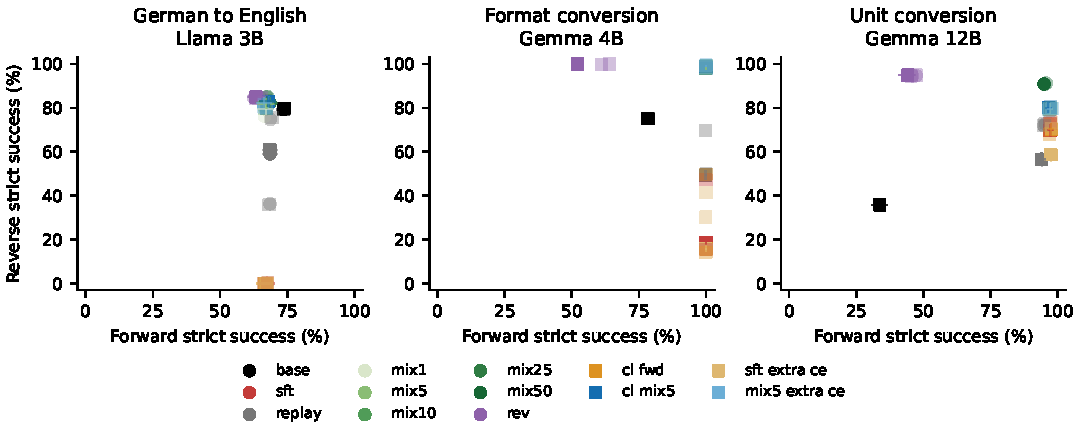
\includegraphics[width=\textwidth]{figures/preservation_frontier.pdf}
\caption{Current preservation frontiers on the fixed reporting panel. Circles show ordinary
SFT/dose campaigns; squares show separately generated contrastive/control campaigns.
Opaque points and marginal cluster-bootstrap intervals are seed-17 results; translucent
points show other training seeds. Contrasts remain paired within each campaign and are
retained with measured runtime/exposure records in the source-backed analysis. The units
null-collapse boundary case is included. No cross-campaign pooled test is implied.}
\label{fig:dose-tradeoff-draft}
\end{figure*}
}{%
\begin{figure}[t]
\centering
\fbox{\parbox{0.9\columnwidth}{\textbf{Draft figure slot: preservation frontier.}
Forward strict success on the horizontal axis; reverse strict success on the vertical axis.
Show base, SFT, replay, reversed-pair doses, and registered contrastive controls in
model--task panels. Add paired intervals, seed variation, and a separate measured-cost panel.
\par\NUM{dose-sentence}}}
\caption{Planned dose--performance--compute summary. No result is drawn in this slot.
Comparisons must share an evaluation campaign; independent campaigns remain separate.
See Appendix~\ref{app:dose-summary} for the reporting protocol.}
\label{fig:dose-tradeoff-draft}
\end{figure}
}

\section{Boundary conditions: information and inverse difficulty}
\label{sec:invertibility}
The format ladder varies whether an inverse is determined, while algebra orientation and
automata probe inverse search difficulty. Several ladder cells fail eligibility and cannot
support tuned-model comparisons; their descriptive base results remain separate.

\paragraph{Two kinds of hardness.} Information loss can prevent a unique inverse even with
unlimited search, whereas a determined inverse can remain computationally difficult. Failed
gates do not distinguish these explanations by themselves.

\section{Is the reverse capability still accessible?}
\label{sec:mechanism}

Four instruments, reported as separate verdicts rather than averaged: they measure different
things, and a disagreement between them is a finding rather than noise.

\paragraph{Elicitation.} The audited reports include both prompt recovery and little recovery
under tested prompts. Best-prompt summaries are exploratory; behavioral recovery does not
prove a specific internal mechanism.
\paragraph{Adapter scaling.} Scaling curves retain forward and reverse success together.
Forward-progress ratios are undefined when the full update has no positive forward gain,
and a curve without reverse loss cannot locate a collapse threshold.
\paragraph{Relearning against a never-had control.} Relearning curves are matched to the
never-had control by model and seed. A small-sample recovery advantage is descriptive evidence
of accessible capability; its uncertainty and starting loss must accompany the comparison.
This is also where the contrast with the reversal curse \citep{berglund2024reversal} becomes
experimental rather than rhetorical: that literature describes capabilities never acquired, and
our never-had control is that case, constructed.
\paragraph{Update repair.} LoRA spectral sweeps are exploratory median-relative filters on
an already low-rank update, with no full-rank noise bulk. Selecting a best threshold on test
success is exploratory. Full-FT projection repair uses a separately registered fixed threshold
and has produced \NUM{audited-fullft-repairs} checkpoint passing saved-weight audits.
The completed fresh generation campaign improves forward and reverse success relative to the
original full-SFT checkpoint. This single exploratory repair does not establish a general remedy.

\paragraph{Explanatory hypothesis and tests.}
Five completed seed-17 diagnostics test task-conditioned output selection
(Appendix~\ref{app:mechanism-sprint}). In formatting and translation collapse cells,
forward SFT reduces reverse gold-over-copy preference and mixed-direction SFT restores it.
Absolute reverse-answer loss worsens in Llama but improves in Gemma translation despite
collapsed generation: answer likelihood and generation are distinct. Final-checkpoint
gradient cosines provide little support for persistent gradient conflict. Local reverse
updates improve held-out loss even in the units null cell, so improvement alone does not
diagnose collapse. Formatting middle-band removals recover reverse success beyond scaling
and random removals matched for retained update norm; all bands and both directions remain
reported. Edit norms are not also matched. These exploratory findings support selective
interference in one cell, without establishing stored knowledge or a universal mechanism.
Direction probes still require input-cue controls; the never-had task differs from the
recovered tasks, and LoRA preserves base weights by construction. Gemma diagnostics exclude
inactive vision factors. The remaining registered diagnostics are running in the background; their pending status supplies no evidence.

\section{Consequences for attribution}
\label{sec:attrib}
We distinguish exposure to both paired sides from an objective-specific generation benefit.

A gain from an auxiliary objective can reflect its directional information, its additional
computation, or the objective itself. Our paired contrastive arms combine forward-only
or mixed-direction CE with symmetric representation alignment. Both sides are encoded
independently, and negatives are drawn only from training data. The contrastive term has no
reverse generation CE, but it still exposes inverse correspondence; it cannot be described as
having no inverse supervision.

\IfFileExists{tables/main_loss_baselines.tex}{% GENERATED by scripts/117_main_results.py
\begin{table*}[!t]
\centering\footnotesize
\textbf{(a) Contrastive objectives and exposure controls}\par\smallskip
\setlength{\tabcolsep}{3pt}
\begin{tabular}{lllrrrrrrrrrr}
\toprule
Task & Model & Dir. & Base & SFT & 5\% & Replay & Rev. & CL-F & CL-M & Shuffle & CE-F+ & CE-M+ \\
\midrule
German $\to$ English & G12B & F & 76.9 & 66.9 & \textcolor{blue!60!black}{\textbf{66.5}} & 67.3 & 1.6 & 66.1 & 66.8 & 66.1 & 66.5 & 66.6 \\
 &  & B & 72.0 & \textcolor{red!70!black}{\textbf{0.2}} & \textcolor{blue!60!black}{\textbf{60.1}} & 56.2 & 66.4 & 0.2 & 60.9 & 0.3 & 0.1 & 60.4 \\
\addlinespace[2pt]
German $\to$ English & G4B & F & 75.4 & 67.7 & \textcolor{blue!60!black}{\textbf{67.4}} & 68.7 & 40.0 & 67.2 & 69.4 & 67.1 & 66.9 & 66.7 \\
 &  & B & 75.8 & \textcolor{red!70!black}{\textbf{0.0}} & \textcolor{blue!60!black}{\textbf{74.4}} & 70.4 & 76.8 & 0.0 & 74.5 & 0.0 & 0.0 & 75.1 \\
\addlinespace[2pt]
German $\to$ English & L8B & F & 74.5 & 64.2 & \textcolor{blue!60!black}{\textbf{65.8}} & 63.9 & 4.7 & 62.8 & 64.5 & 63.8 & 62.8 & 65.1 \\
 &  & B & 73.0 & \textcolor{red!70!black}{\textbf{16.5}} & \textcolor{blue!60!black}{\textbf{68.9}} & 64.3 & 75.1 & 0.0 & 67.7 & 0.0 & 18.2 & 69.6 \\
\addlinespace[2pt]
German $\to$ English & L3B & F & 73.7 & 67.3 & \textcolor{blue!60!black}{\textbf{67.0}} & 68.5 & 63.4 & 66.5 & 68.0 & 66.7 & 67.0 & 66.4 \\
 &  & B & 79.7 & \textcolor{red!70!black}{\textbf{0.0}} & \textcolor{blue!60!black}{\textbf{82.0}} & 61.0 & 84.9 & 0.0 & 82.9 & 0.1 & 0.0 & 82.2 \\
\addlinespace[2pt]
Format conversion & G4B & F & 78.3 & 100.0 & \textcolor{blue!60!black}{\textbf{99.9}} & 99.8 & 52.2 & 100.0 & 99.9 & 99.9 & 99.9 & 100.0 \\
 &  & B & 75.1 & \textcolor{red!70!black}{\textbf{18.7}} & \textcolor{blue!60!black}{\textbf{98.0}} & 49.3 & 100.0 & 15.8 & 99.0 & 45.0 & 15.8 & 99.1 \\
\addlinespace[2pt]
Format conversion & L8B & F & 80.2 & 99.5 & \textcolor{blue!60!black}{\textbf{99.9}} & 99.8 & 2.2 & 100.0 & 99.8 & 99.7 & 100.0 & 99.9 \\
 &  & B & 69.0 & \textcolor{red!70!black}{\textbf{0.0}} & \textcolor{blue!60!black}{\textbf{98.7}} & 32.1 & 99.9 & 2.2 & 99.2 & 0.0 & 0.0 & 98.7 \\
\addlinespace[2pt]
Format conversion & L3B & F & 60.6 & 99.7 & \textcolor{blue!60!black}{\textbf{99.9}} & 98.9 & 27.0 & 99.6 & 99.6 & 99.7 & 99.2 & 99.7 \\
 &  & B & 51.4 & \textcolor{red!70!black}{\textbf{0.4}} & \textcolor{blue!60!black}{\textbf{96.0}} & 25.6 & 99.4 & 0.1 & 96.0 & 0.8 & 0.6 & 94.2 \\
\addlinespace[2pt]
Unit conversion & G12B & F & 33.7 & 97.1 & \textcolor{blue!60!black}{\textbf{97.0}} & 94.0 & 44.1 & 97.6 & 96.5 & 97.5 & 97.4 & 97.1 \\
 &  & B & 35.8 & 69.8 & \textcolor{blue!60!black}{\textbf{79.4}} & 56.5 & 94.9 & 70.3 & 80.1 & 74.1 & 58.7 & 79.6 \\
\bottomrule
\end{tabular}
\par\medskip\textbf{(b) Other auxiliary objectives}\par\smallskip
\setlength{\tabcolsep}{3pt}
\begin{tabular}{lllrrrrrr}
\toprule
Task & Model & Dir. & Base & SFT & 5\% & CFT & Unlikelihood & Round-trip \\
\midrule
English $\to$ German & L8B & F & 71.1 & 73.1 & \textcolor{blue!60!black}{\textbf{73.0}} & -- & 74.0 & -- \\
 &  & B & 74.2 & 58.7 & \textcolor{blue!60!black}{\textbf{69.2}} & -- & 0.1 & -- \\
\addlinespace[2pt]
English $\to$ German & L3B & F & 79.7 & 84.8 & \textcolor{blue!60!black}{\textbf{85.4}} & -- & 85.1 & -- \\
 &  & B & 72.8 & 63.6 & \textcolor{blue!60!black}{\textbf{68.8}} & -- & 0.0 & -- \\
\addlinespace[2pt]
Code transformation & L3B & F & 38.0 & 81.4 & \textcolor{blue!60!black}{\textbf{84.2}} & 84.1 & -- & -- \\
 &  & B & 32.0 & \textcolor{red!70!black}{\textbf{3.6}} & \textcolor{blue!60!black}{\textbf{75.4}} & 6.7 & -- & -- \\
\addlinespace[2pt]
Question $\to$ SQL & L8B & F & 62.0 & 72.1 & \textcolor{blue!60!black}{\textbf{71.9}} & -- & -- & 71.3 \\
 &  & B & 54.9 & 51.3 & \textcolor{blue!60!black}{\textbf{57.8}} & -- & -- & 58.8 \\
\addlinespace[2pt]
Question $\to$ SQL & L3B & F & 49.1 & 62.3 & \textcolor{blue!60!black}{\textbf{61.0}} & -- & -- & 61.5 \\
 &  & B & 51.5 & \textcolor{red!70!black}{\textbf{23.3}} & \textcolor{blue!60!black}{\textbf{55.2}} & -- & -- & 48.2 \\
\bottomrule
\end{tabular}
\caption{Strict success (\%); F/B denotes forward/backward. Blue highlights small reversed-pair doses; red highlights SFT backward success at most half the same-pass base (a descriptive threshold). All eligible original contrastive and audited auxiliary-objective cells at fixed seed 17. Each task/model row pair uses its own fresh evaluation pass and base; scores across campaigns are not treatment contrasts. L/G denotes Llama/Gemma; B denotes billions of parameters. The $5\%$ column is ordinary reversed-pair SFT. CL-F/M adds alignment to forward/mixed-direction CE; Shuffle randomizes positive pairs; CE-F+/M+ adds CE as an exposure proxy; CFT is conflict-aware fine-tuning. Dashes denote untested objectives. Failed gates, other seeds and paired intervals remain in the appendix/audit.}\label{tab:main-loss-baselines}
\end{table*}
}{}
Table~\ref{tab:main-loss-baselines} reports fresh, complete passes for the registered
contrastive comparison and auxiliary objectives that pass the current exposure/withdrawal
audit. Each row pair has its own base; numerical differences across evaluation campaigns
are not treatment effects. The contrastive grid currently completes
\NUM{contrastive-completed-cells} of \NUM{contrastive-planned-cells} registered
model--task--seed cells. Appendix~\ref{app:complete-main-comparisons} retains every
registered primary contrast, per-seed uncertainty and exposure control.

Forward-only contrastive alignment provides no consistent benefit over extra-CE or shuffled
controls. In the reference code cell, conflict-aware fine-tuning falls well short of $5\%$
reversed-pair SFT on backward generation; forward-only unlikelihood also fails to preserve
backward translation in the audited cells. This supports trying backward examples before
adding an auxiliary objective. It does not establish that every loss baseline is inferior:
mixed-direction alignment sometimes beats $5\%$ SFT, and round-trip training wins backward
success in one SQL cell while trading forward performance. Extra-CE controls match an
exposure proxy, not identical measured FLOPs. An interval spanning zero does not establish
equivalence, and degenerate intervals at a generation floor require particular caution.

\paragraph{New-domain eligibility.}
The \NUM{failed-new-domain-gates} original small-model task--model gates failed the unchanged
eligibility criteria (Table~\ref{tab:domain-gates-snapshot}). Complete test-set gates and
scorer audits are retained. No tuned pilot is admitted for these failed cells. Explicit-output
variants reuse their corpora; they are prompt diagnostics and cannot be counted as independent
new-domain successes. The \NUM{failed-explicit-domain-gates} completed explicit-format
gates also fail the unchanged criteria. Larger-model feasibility gates on the original
tasks are separately registered. Gemma12B passes the unit-conversion gate and completes
valid replicated campaigns (Table~\ref{tab:generality-snapshot}). Forward-only SFT improves
both directions; this is retained as a replicated null-collapse result. Replication seeds are admitted by validity,
independently of effect sign. Llama8B also passes Python--C++ translation after a technical parser retry; its pilot is
evaluated under the registered same-pass protocol. Boolean gates remain failed, with correctness criteria unchanged.
\IfFileExists{tables/domain_gates_snapshot.tex}{\begin{table*}[t]
\centering\small
\begin{tabular}{lllll}
\toprule
Task & Model & Forward & Reverse & Eligibility \\
\midrule
units & llama32-3b & 0.4 & 1.9 & Fail \\
units & gemma3-4b & 37.6 & 3.5 & Fail \\
logic & llama32-3b & 0.0 & 0.0 & Fail \\
logic & gemma3-4b & 0.0 & 0.0 & Fail \\
py\_cpp & llama32-3b & 78.6 & 74.1 & Fail \\
py\_cpp & gemma3-4b & 5.1 & 99.9 & Fail \\
\bottomrule
\end{tabular}
\caption{Initial task feasibility: base-model strict success in percent. Comparisons require adequate performance in both directions and a scorer that rejects copied outputs. Explicit-output diagnostics use the same semantic splits and are separate exploratory variants.}
\label{tab:domain-gates-snapshot}
\end{table*}
}{}
\IfFileExists{tables/generality_snapshot.tex}{\begin{table*}[t]
\centering\small
\begin{tabular}{llllll}
\toprule
Task & Model & Seed & Arm & Forward & Reverse \\
\midrule
py\_cpp & llama31-8b & 17 & base & 85.9 & 100.0 \\
py\_cpp & llama31-8b & 17 & sft & 100.0 & 0.0 \\
py\_cpp & llama31-8b & 17 & mix50 & 100.0 & 48.7 \\
py\_cpp & llama31-8b & 17 & replay & 100.0 & 97.6 \\
py\_cpp & llama31-8b & 17 & rev & 0.0 & 0.0 \\
py\_cpp & llama31-8b & 42 & base & 84.2 & 100.0 \\
py\_cpp & llama31-8b & 42 & sft & 100.0 & 0.0 \\
py\_cpp & llama31-8b & 42 & mix50 & 1.7 & 0.0 \\
py\_cpp & llama31-8b & 42 & replay & 99.9 & 99.5 \\
py\_cpp & llama31-8b & 42 & rev & 0.0 & 0.0 \\
units & gemma3-12b & 1234 & base & 33.7 & 35.8 \\
units & gemma3-12b & 1234 & sft & 96.9 & 72.7 \\
units & gemma3-12b & 1234 & mix50 & 95.1 & 90.7 \\
units & gemma3-12b & 1234 & replay & 94.8 & 71.9 \\
units & gemma3-12b & 1234 & rev & 47.3 & 94.7 \\
units & gemma3-12b & 17 & base & 33.7 & 35.8 \\
units & gemma3-12b & 17 & sft & 97.4 & 70.0 \\
units & gemma3-12b & 17 & mix50 & 94.9 & 90.9 \\
units & gemma3-12b & 17 & replay & 94.0 & 56.6 \\
units & gemma3-12b & 17 & rev & 44.0 & 95.0 \\
units & gemma3-12b & 42 & base & 33.7 & 35.8 \\
units & gemma3-12b & 42 & sft & 97.3 & 73.7 \\
units & gemma3-12b & 42 & mix50 & 95.7 & 91.3 \\
units & gemma3-12b & 42 & replay & 95.5 & 72.7 \\
units & gemma3-12b & 42 & rev & 45.9 & 94.6 \\
py\_cpp & llama31-8b & 1234 & base & 84.2 & 100.0 \\
py\_cpp & llama31-8b & 1234 & sft & 100.0 & 0.0 \\
py\_cpp & llama31-8b & 1234 & mix50 & 100.0 & 0.2 \\
py\_cpp & llama31-8b & 1234 & replay & 95.8 & 97.9 \\
py\_cpp & llama31-8b & 1234 & rev & 0.0 & 0.0 \\
\bottomrule
\end{tabular}
\caption{Eligible larger-model generality campaigns: strict success in percent, with all arms and the base evaluated in one fresh pass per model/task/seed. The completed unit-conversion replications improve both directions under SFT and are retained null-collapse boundary cases. Additional eligible campaigns enter this table after validated analysis.}
\label{tab:generality-snapshot}
\end{table*}
}{}

\paragraph{Full-weight checks.}
Full-FT training is complete; \NUM{fullft-completed-cells} of \NUM{fullft-planned-cells}
validated evaluation campaigns are complete in the current snapshot.
Full checkpoints require isolated engines, unlike the single-engine multi-LoRA comparisons.
Their newly generated campaigns use the same instances, messages, tokenizer, and scoring
settings but span engine restarts. We record this layout and interpret small differences
against the decoding floor. Projection-matrix spectral repair is exploratory; it does not
assume a validated noise model. Repair results require joint reverse/forward interpretation.
\IfFileExists{tables/fullft_snapshot.tex}{\begin{table*}[t]
\centering\small
\begin{tabular}{llllll}
\toprule
Task & Seed & Direction & Base & Full SFT & Full mix5 \\
\midrule
code & 17 & forward & 37.9 & 70.0 & 70.7 \\
code & 17 & reverse & 31.9 & 2.0 & 65.9 \\
mt\_de-en & 17 & forward & 73.3 & 70.9 & 72.0 \\
mt\_de-en & 17 & reverse & 80.1 & 72.8 & 83.6 \\
mt\_en-de & 17 & forward & 80.1 & 87.0 & 86.6 \\
mt\_en-de & 17 & reverse & 72.9 & 69.9 & 72.4 \\
mt\_en-zh & 17 & forward & 73.9 & 79.1 & 79.2 \\
mt\_en-zh & 17 & reverse & 75.9 & 66.9 & 71.8 \\
mt\_zh-en & 17 & forward & 76.3 & 74.2 & 73.9 \\
mt\_zh-en & 17 & reverse & 73.8 & 70.2 & 78.5 \\
sql & 17 & forward & 49.3 & 60.5 & 59.7 \\
sql & 17 & reverse & 50.4 & 18.7 & 55.1 \\
\bottomrule
\end{tabular}
\caption{Completed Llama3B full-weight campaign rates in percent, with forward and reverse retention. Checkpoints use isolated engines and identical held-out instances; these comparisons span engine restarts. Paired intervals are recorded in followup contrasts. An empty body means no validated full campaign has completed.}
\label{tab:fullft-snapshot}
\end{table*}
}{}

\section{Related work}
\label{sec:related}

Prior directional degradation and reverse training are established starting points. Our
contribution is the joint preservation comparison and controlled attribution, qualified by
failed gates and replicated null-collapse results.

\paragraph{Directional degradation and reverse training.}
\citet{nikiema2025contrastive} study cognitive specialization in code transformation;
\citet{zhu2024finetuning} examine direction-dependent degradation in translation. We ask
how preservation varies across domains, doses, models, and objectives. Program-execution
reasoning also exhibits directional asymmetry \citep{hasanov2026pathnottaken}, motivating
cell-specific measurement of starting reverse capability. The reversal curse concerns
capabilities never acquired \citep{berglund2024reversal}; reverse training addresses this
at the data level under data- and compute-matched comparisons
\citep{golovneva2024reversetraining}. Our relearning experiment compares a collapsed model
with a model-matched never-had control. Replacement mixtures hold instances and steps fixed
while auditing realized exposure.

\paragraph{Forgetting and rehearsal.}
Broader forgetting after fine-tuning \citep{luo2023forgetting} and differences between LoRA
and full fine-tuning \citep{biderman2024lora} motivate our general-ability and full-weight
controls; they do not bound directional loss in these tasks. Rehearsal can preserve earlier
performance \citep{scialom2022rehearsal}. Generic replay at the registered replacement share
tests whether directional content adds preservation beyond that explanation. Concentration
of inverse loss relative to general ability remains a separate empirical question.

\paragraph{Recovery and task inference.}
Wrapper and offset accounts of fine-tuning \citep{jain2024wrapper,lee2024dpo}, update filtering
\citep{spectral2026unforgetting}, and skewed task inference \citep{kotha2024forgetting}
motivate distinct recovery instruments. Our directional tests include a never-had control,
both-direction retention, and fixed-threshold exploratory repair. Behavioral recovery does
not identify a unique internal mechanism, and bidirectional behavior need not imply a unified
representation \citep{latentgen2026illusion}.

\paragraph{Attributing objective gains.}
Data mixtures and reporting choices can confound objective attribution
\citep{longpre2023flan,lipton2018troubling}. RevThink adds backward questions and reasoning
\citep{chen2025revthink}; its cross-entropy components illustrate why directional exposure
must be controlled when assessing a bidirectional objective. Our paired contrastive comparison
includes reversed-pair SFT, extra-CE proxies, and shuffled positives, measuring generation in
both directions. These controls test the scope of an objective-specific gain without assuming
that auxiliary objectives are universally unnecessary.

\section{Conclusion}
Forward-only SFT can improve the trained task while damaging an existing backward task.
Small-dose reversed-pair SFT directly addresses that failure with ordinary cross-entropy:
$1\%$ reversal gives substantial backward recovery with little forward change in the
reference formatting and code cells. The complete tables retain harder tradeoffs, nulls,
and objective-specific gains. Evaluate both directions and establish this simple baseline
before attributing preservation to a more complex loss. Recovery evidence motivates
selective interference as a hypothesis, without proving memory erasure or a universal cause.

% ---------------------------------------------------------------------------
% ARR requires a Limitations section. It is unnumbered and does not count against the page
% limit, which is not a reason to make it short.
\section*{Limitations}
\label{sec:limitations}

\paragraph{Where the repair does not reach.} Reversed-pair training cannot recover information
absent from an input. Our failed new-domain gates also limit generality beyond established tasks.

\paragraph{Scale.} The full arm set runs at 1--4B with three seeds; only core arms run at
8--12B with two where eligible in the original grid. Separately registered larger-model
extensions add replication and objective controls in selected cells; coverage remains uneven.
This does not establish scaling to larger models.

\paragraph{LoRA.} Most arms use LoRA. Prior work reports different retention under full
fine-tuning \citep{biderman2024lora}; this does not guarantee a conservative directional-loss
estimate in our tasks. The full-FT check covers only the registered Llama 3B seed-17 cells;
it cannot bound directional loss across other models or training recipes.

\paragraph{Resolution of the dose ladder.} Adjacent rungs differ by a couple of points, which
our evaluation sets may not separate reliably. Final dose claims require intervals and seed
ranges; an interval spanning zero does not establish equivalence.

\paragraph{Criteria with a model in them.} Two directions are scored by round-tripping through a
frozen model rather than by execution. Each reports that model's own accuracy on the references
as the criterion's ceiling where measured. Extractor/parser errors can reject valid generations;
the D2T measurement is still undergoing validation.

\paragraph{Languages and domains.} The original code-transformation cell is Python only;
the translation cells cover two
language pairs, both with English on one side. Synthetic task variants do not establish natural
code or unrestricted reasoning generality, and reused semantic corpora are not independent evidence.
Independent transfer retains failed eligibility boundaries; completed prompt and training-recipe
tests retain adverse and null findings (Appendices~\ref{app:independent-transfer} and~\ref{app:robustness}).

% Acknowledgments belong only in the camera-ready version.
\bibliography{refs}

\appendix
\section{Complete comparison counts and objective contrasts}
\label{app:complete-main-comparisons}
The main tables show strict success percentages for a fixed reference seed. The following
inventory covers the broader audited grid; contrastive tables retain all registered paired
contrasts with their uncertainty and controls. Highlighting in the main tables identifies
arms and the descriptive collapse threshold, not statistical significance.
\IfFileExists{tables/core_inventory.tex}{\begin{table*}[t]
\centering\small
\begin{tabular}{llll}
\toprule
Model & Task orientations & Cells & Threshold met \\
\midrule
gemma3-12b & 7 & 14 & 8 \\
gemma3-4b & 7 & 21 & 14 \\
llama31-8b & 6 & 12 & 7 \\
llama32-3b & 11 & 32 & 18 \\
olmo2-1b & 4 & 12 & 5 \\
\bottomrule
\end{tabular}
\caption{Audited model--task--seed cells. Threshold met means SFT reverse strict success is at most half the same-pass base rate. Counts are descriptive and are not independent task counts or pooled significance tests.}
\label{tab:core-inventory}
\end{table*}
}{}
\begin{figure}[t]
\centering
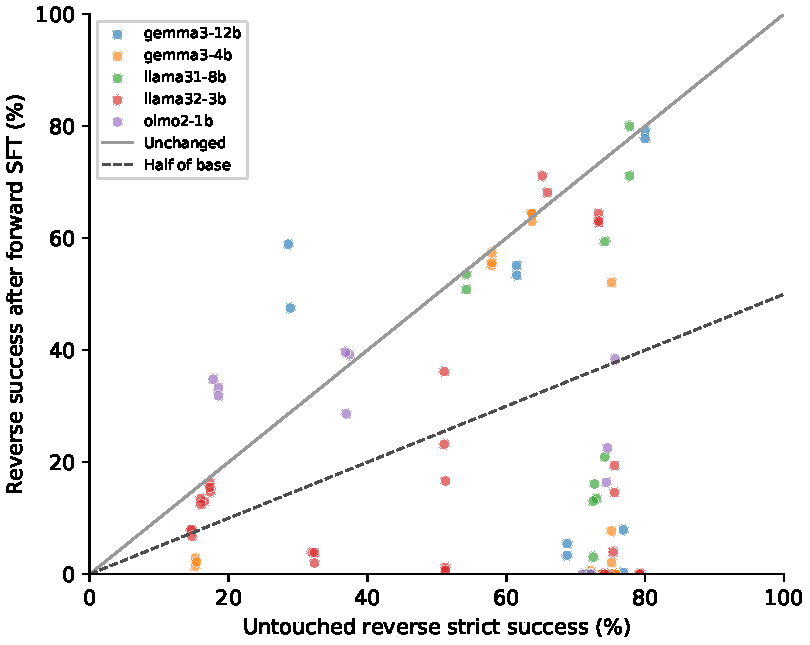
\includegraphics[width=\columnwidth]{figures/directional_loss_snapshot.pdf}
\caption{Audited model--task--seed cells, each using a same-pass base and SFT. The dashed
line marks half the base rate. Repeated tasks and seeds are not independent observations.}
\label{fig:directional-loss-snapshot}
\end{figure}
\IfFileExists{tables/contrastive_snapshot.tex}{\begin{table*}[t]
\centering\small
\begin{tabular}{lllll}
\toprule
Task & Model & Seed & $\Delta$ CL-fwd versus SFT & $\Delta$ CL-mix5 versus mix5 \\
\midrule
fmt & gemma3-4b & 17 & -2.88 [-3.88, -1.96] & +1.08 [+0.32, +1.88] \\
fmt & gemma3-4b & 42 & -1.28 [-1.96, -0.64] & -1.04 [-1.80, -0.32] \\
fmt & gemma3-4b & 1234 & +2.36 [+1.60, +3.20] & -0.32 [-0.92, +0.24] \\
fmt & llama31-8b & 17 & +2.24 [+1.52, +3.04] & +0.48 [-0.12, +1.12] \\
fmt & llama31-8b & 42 & -33.12 [-35.48, -30.64] & +0.40 [-0.20, +1.00] \\
fmt & llama31-8b & 1234 & +0.00 [+0.00, +0.00] & -0.72 [-1.52, +0.12] \\
fmt & llama32-3b & 17 & -0.24 [-0.56, +0.04] & +0.00 [-1.12, +1.12] \\
fmt & llama32-3b & 42 & -1.48 [-2.12, -0.92] & +1.68 [+0.52, +2.88] \\
fmt & llama32-3b & 1234 & -0.52 [-1.00, -0.04] & +4.44 [+3.08, +5.84] \\
mt\_de-en & gemma3-12b & 17 & +0.00 [+0.00, +0.00] & +0.79 [-1.78, +3.56] \\
mt\_de-en & gemma3-12b & 42 & -0.10 [-0.40, +0.00] & +0.59 [-2.08, +3.26] \\
mt\_de-en & gemma3-12b & 1234 & +0.00 [+0.00, +0.00] & +0.69 [-1.68, +3.16] \\
mt\_de-en & gemma3-4b & 17 & +0.00 [+0.00, +0.00] & +0.10 [-2.27, +2.27] \\
mt\_de-en & gemma3-4b & 42 & +0.00 [+0.00, +0.00] & +0.40 [-2.08, +2.77] \\
mt\_de-en & gemma3-4b & 1234 & +0.00 [+0.00, +0.00] & -0.30 [-2.47, +2.17] \\
mt\_de-en & llama31-8b & 17 & -16.50 [-19.47, -13.64] & -1.19 [-4.05, +1.88] \\
mt\_de-en & llama31-8b & 42 & -13.54 [-16.50, -11.07] & -0.40 [-3.26, +2.57] \\
mt\_de-en & llama31-8b & 1234 & -23.32 [-26.78, -19.96] & -1.28 [-4.35, +1.58] \\
mt\_de-en & llama32-3b & 17 & +0.00 [+0.00, +0.00] & +0.89 [-1.38, +3.26] \\
mt\_de-en & llama32-3b & 42 & +0.00 [+0.00, +0.00] & +2.47 [+0.00, +5.04] \\
mt\_de-en & llama32-3b & 1234 & -0.10 [-0.40, +0.00] & +0.10 [-2.57, +2.87] \\
units & gemma3-12b & 17 & +0.50 [-1.70, +2.80] & +0.70 [-0.90, +2.30] \\
units & gemma3-12b & 42 & -1.40 [-2.70, -0.20] & +0.40 [-1.10, +2.00] \\
units & gemma3-12b & 1234 & -4.90 [-7.00, -3.10] & +0.50 [-0.90, +1.90] \\
\bottomrule
\end{tabular}
\caption{Completed exploratory reverse-generation contrasts (percentage points), with 99\% paired cluster-bootstrap intervals. Five primary contrasts are adjusted within each cell; no adjustment across cells. All completed original and scale/domain-extension comparisons are included; excluded cells remain eligibility boundaries rather than tuned comparisons.}
\label{tab:contrastive-snapshot}
\end{table*}
}{}
\IfFileExists{tables/contrastive_controls.tex}{\begin{table*}[t]
\centering\small
\begin{tabular}{llllll}
\toprule
Task & Model & Seed & CL-fwd vs extra CE & CL-fwd vs shuffled & CL-mix5 vs extra CE \\
\midrule
fmt & Gemma 4B & 17 & +0.04 [-0.84, +0.96] & -29.20 [-31.80, -26.72] & -0.08 [-0.72, +0.56] \\
fmt & Gemma 4B & 42 & -16.04 [-18.00, -14.20] & -19.44 [-21.52, -17.48] & -0.44 [-1.28, +0.44] \\
fmt & Gemma 4B & 1234 & +8.20 [+6.80, +9.64] & -22.16 [-25.08, -19.24] & -0.60 [-1.24, +0.00] \\
fmt & Llama 3B & 17 & -0.48 [-0.96, -0.08] & -0.68 [-1.16, -0.24] & +1.76 [+0.56, +2.96] \\
fmt & Llama 3B & 42 & -1.76 [-2.48, -1.12] & -3.40 [-4.32, -2.52] & +0.64 [-0.44, +1.68] \\
fmt & Llama 3B & 1234 & -0.36 [-0.88, +0.12] & +0.28 [+0.08, +0.60] & +2.76 [+1.48, +4.00] \\
mt\_de-en & Gemma 4B & 17 & +0.00 [+0.00, +0.00] & +0.00 [+0.00, +0.00] & -0.59 [-2.77, +1.58] \\
mt\_de-en & Gemma 4B & 42 & +0.00 [+0.00, +0.00] & +0.00 [+0.00, +0.00] & +0.00 [-2.27, +2.27] \\
mt\_de-en & Gemma 4B & 1234 & +0.00 [+0.00, +0.00] & +0.00 [+0.00, +0.00] & +1.09 [-1.09, +3.36] \\
mt\_de-en & Llama 3B & 17 & +0.00 [+0.00, +0.00] & -0.10 [-0.40, +0.00] & +0.69 [-1.68, +3.16] \\
mt\_de-en & Llama 3B & 42 & +0.00 [+0.00, +0.00] & -0.10 [-0.40, +0.00] & +1.78 [-0.59, +4.25] \\
mt\_de-en & Llama 3B & 1234 & -0.10 [-0.40, +0.00] & -0.10 [-0.40, +0.00] & -0.69 [-3.26, +1.88] \\
\bottomrule
\end{tabular}
\caption{The remaining three registered primary reverse-generation contrasts, in percentage points with 99\% paired cluster-bootstrap intervals. Together with Table~\ref{tab:contrastive-snapshot}, these display all five primary comparisons for every completed cell. Extra CE is an exposure/compute proxy, not matched measured FLOPs. Degenerate zero intervals at an observed generation floor do not establish equivalence. Results remain exploratory; new scale/domain extensions are pending.}
\label{tab:contrastive-controls}
\end{table*}
}{}
% Paper-completion protocols registered in Amendment 50, October 8, 2026.
% Fill measured outcomes through source-backed generators, never by hand.
\section{Additional evaluations, methods, and reporting audit}
\label{app:planned-evaluations}

This appendix reports the exploratory additions registered before their measurements,
their completed findings, and the boundaries that prevented eligible tuned comparisons.
Allocation-local engineering smokes preceded production admission; passing a smoke alone
did not establish a scientific result. The retained diagnostic subset comprises the five
completed campaigns specified in Amendment54; broader registered diagnostics remain unmeasured.
Failed gates and the replicated Gemma12B unit-conversion null-collapse result remain visible.
\IfFileExists{tables/paper_finish_protocol.tex}{\begin{table*}[t]
\centering\small
\begin{tabular}{llll}
\toprule
Registered evaluation & Model/task cells & Training seeds & Campaigns \\
\midrule
General probes & 3 & 17,42,1234 & 9 \\
Prompt/template tests & 4 & 17,42,1234 & 12 \\
Independent transfer & 2 & 17,42,1234 & 6 \\
Recipe evaluations & 2 & 17,42,1234 & 6 \\
\bottomrule
\end{tabular}
\caption{Frozen paper-completion panel. Probe corpora retain 541 IFEval prompts and 1319 GSM8K questions; independent transfer retains 1688 OPUS translation pairs. Synthetic magnitude/template tests retain 1000 instances each. Recipe packs train 48 new adapters in isolated directories. Counts are planned workloads and audited corpus sizes, not completed results.}
\label{tab:paper-finish-protocol}
\end{table*}
}{}

\subsection{Paired data and reference training recipe}
\label{app:reference-methods}

Each task supplies fixed training, validation, and test pairs. Content and pair-identity
overlap checks exclude held-out test material during corpus construction; validation is
not used to select a preferred test result. Opposite orientations of a task share the
underlying task family. The reference recipe and actual corpus/trainer counts are reported
in Table~\ref{tab:reference-methods}; smaller factual-relation and execution corpora are
retained at their actual size. Seed-specific partitions define reversed-pair replacement.
Training summaries retain realized supervised-token exposure and length filtering, rather
than equating pair count with tokens. Every reported tuned comparison includes a freshly
evaluated base and all declared arms on the same retained instance set.
% GENERATED by scripts/118_manuscript_completion.py
\paragraph{Recorded reference recipe.}
The main-table Llama3B experiments use the common training recipe: LoRA rank $32$, scaling $64$, dropout $0.05$, learning rate $0.0001$, $3$ epochs, effective batch $64$, and maximum sequence length $2048$ tokens. The scheduler is cosine with warm-up fraction $0.03$, weight decay $0$ and gradient clipping $1$. Training uses bfloat16 and final checkpoints without intermediate checkpoint selection. LoRA targets query, key, value and output attention projections and the gate, up and down MLP projections. Allocation-specific microbatches and accumulation retain the recorded effective batch. Full-weight and robustness variants are separate recipes, not substitutions for this reference.
\begin{table*}[t]
\centering\footnotesize
\setlength{\tabcolsep}{4pt}
\begin{tabular}{lrrrrrrr}
\toprule
Task orientation & Train & Val. & Test & Retained & Eval. & Steps & Batch $\times$ accum. \\
\midrule
German $\to$ English & 6500 & 500 & 1012 & 6500 & 1012 & 306 & $16\times4$ \\
English $\to$ German & 6500 & 500 & 1012 & 6500 & 1012 & 306 & $4\times16$ \\
English $\to$ Chinese & 6500 & 500 & 1012 & 6500 & 1012 & 306 & $4\times16$ \\
Chinese $\to$ English & 6500 & 500 & 1012 & 6500 & 1012 & 306 & $4\times16$ \\
Code transformation & 6500 & 500 & 2060 & 6499 & 2060 & 306 & $4\times16$ \\
Question $\to$ SQL & 6499 & 500 & 1034 & 6499 & 1034 & 306 & $16\times4$ \\
Format conversion & 6500 & 500 & 2500 & 6500 & 2500 & 306 & $16\times4$ \\
Factual relations & 504 & 69 & 135 & 504 & 135 & 24 & $16\times4$ \\
Polynomial expansion & 6500 & 500 & 2500 & 6500 & 2500 & 306 & $4\times16$ \\
Polynomial factorization & 6500 & 500 & 2500 & 6500 & 2500 & 306 & $4\times16$ \\
Execution prediction & 302 & 100 & 200 & 302 & 200 & 15 & $16\times4$ \\
\bottomrule
\end{tabular}
\caption{Built paired-corpus sizes and recorded forward-SFT training/evaluation counts for the main-table reference campaigns. Train/validation/test counts are verified against the current frozen JSONL files; retained rows, steps and batch shapes come from each saved training manifest/summary. These are distinct provenance records: the code campaign retains fewer training rows than the current built corpus. Historical training data bytes are not inferred from a current file hash. Eval. counts paired instances per arm and direction. Opposite task orientations reuse task families; they are not independent datasets.}
\label{tab:reference-methods}
\end{table*}


\subsection{Dose, forward retention, and computational cost}
\label{app:dose-summary}

The main figure plots forward and reverse strict success for the base model, forward SFT,
generic replay, available reversed-pair doses, and contrastive/control arms. Panels retain
model, task orientation, and seed identity. Arms lacking a common evaluation campaign are not
connected as paired observations. The units boundary case is shown alongside collapse cells.
Repeated passes use the latest validated completion time, with earlier passes retained in the
audit; selection never uses effect sign.

Paired contrasts use the domain's instance/cluster unit. Training-seed variation is separate:
resampling test instances does not measure training variability. No aggregate pools cells as
independent domains. The dose knee uses the criterion in \S\ref{sec:dose}; overlapping
intervals do not establish equivalence.

The cost table reports available trainer runtime, optimizer steps, and CE-corpus tokens.
Auxiliary encoded-side exposure is retained separately in the analysis. Missing timing,
GPU-type, queue-time, or exposure records remain unavailable. Additional CE is the declared
proxy; corpus token counts alone do not establish matched objective FLOPs or wall time.
\IfFileExists{tables/preservation_summary.tex}{\begin{table*}[t]
\centering\small
\begin{tabular}{llllll}
\toprule
Task & Model & Seed & Arm & Forward (\%) & Reverse (\%) \\
\midrule
mt\_de-en & llama32-3b & 17 & base & 73.7 & 79.2 \\
mt\_de-en & llama32-3b & 17 & sft & 67.1 & 0.0 \\
mt\_de-en & llama32-3b & 17 & replay & 68.6 & 59.0 \\
mt\_de-en & llama32-3b & 17 & mix5 & 67.4 & 82.0 \\
mt\_de-en & llama32-3b & 17 & mix50 & 67.4 & 82.9 \\
units & gemma3-12b & 17 & base & 33.7 & 35.8 \\
units & gemma3-12b & 17 & sft & 97.4 & 70.0 \\
units & gemma3-12b & 17 & replay & 94.0 & 56.6 \\
units & gemma3-12b & 17 & mix50 & 94.9 & 90.9 \\
\bottomrule
\end{tabular}
\caption{Representative seed-17 preservation rates. Each model/task row set comes from one complete campaign. Additional doses, seed variation, paired intervals and measured cost records are retained in the source-backed analysis. The units boundary case is included independently of effect sign.}
\label{tab:preservation-summary}
\end{table*}
}{}
\IfFileExists{tables/preservation_costs.tex}{\begin{table*}[t]
\centering\small
\begin{tabular}{llllll}
\toprule
Task & Model & Arm & Minutes & Steps & CE corpus tokens \\
\midrule
mt\_de-en & llama32-3b & sft & 8.9 & 306 & 1096262 \\
mt\_de-en & llama32-3b & mix5 & 8.9 & 306 & 1096262 \\
mt\_de-en & llama32-3b & mix50 & 9.0 & 306 & 1096262 \\
mt\_de-en & llama32-3b & replay & 8.9 & 306 & 1096110 \\
mt\_de-en & llama32-3b & sft & 8.9 & 306 & 1096262 \\
mt\_de-en & llama32-3b & mix5 & 8.9 & 306 & 1096262 \\
mt\_de-en & llama32-3b & replay & 8.9 & 306 & 1096110 \\
mt\_de-en & llama32-3b & cl\_fwd & 241.9 & 306 & 1096262 \\
mt\_de-en & llama32-3b & cl\_mix5 & 62.2 & 306 & 1096262 \\
mt\_de-en & llama32-3b & sft\_extra\_ce & 123.2 & 306 & 1096262 \\
mt\_de-en & llama32-3b & mix5\_extra\_ce & 119.1 & 306 & 1096262 \\
fmt & gemma3-4b & sft & 30.6 & 306 & 1927990 \\
fmt & gemma3-4b & mix5 & 30.7 & 306 & 1927882 \\
fmt & gemma3-4b & replay & 30.2 & 306 & 1927978 \\
fmt & gemma3-4b & cl\_fwd & 194.3 & 306 & 1927990 \\
fmt & gemma3-4b & cl\_mix5 & 193.5 & 306 & 1927882 \\
fmt & gemma3-4b & sft\_extra\_ce & 191.3 & 306 & 1927990 \\
fmt & gemma3-4b & mix5\_extra\_ce & 194.0 & 306 & 1927882 \\
units & gemma3-12b & sft & 21.6 & 306 & 788819 \\
units & gemma3-12b & mix50 & 22.1 & 306 & 788819 \\
units & gemma3-12b & replay & 21.5 & 306 & 799547 \\
\bottomrule
\end{tabular}
\caption{Recorded seed-17 trainer runtimes (minutes), optimizer steps, and sequence tokens in the tokenized CE corpus (before epoch repetition). Auxiliary encoded-side exposure remains separately recorded in the analysis; these token counts are not total objective FLOPs. Runtime varies with GPU/training layout and is not a claim of matched wall time. Missing measurements are unavailable, never inferred.}
\label{tab:preservation-costs}
\end{table*}
}{}
\paragraph{Scoped finding.} On the representative translation campaign, reversed-pair SFT
preserves reverse behavior with nearly unchanged forward task performance relative to forward
SFT (Table~\ref{tab:preservation-summary}). Generic replay recovers less reverse performance
in that campaign. The units case improves both ways under ordinary SFT; robustness results
show that preservation and forward costs depend on task and recipe. Recorded budgets support
within-recipe comparisons, not matched wall-time claims across different objectives.

\subsection{General ability and overlap controls}
\label{app:general-probes}

The fixed panel is German-to-English/Llama3B, format conversion/Gemma4B, and units/Gemma12B.
Each campaign compares base, SFT, replay, mixed-direction SFT, forward-only and mixed-direction
contrastive arms, and their additional-CE controls. The auxiliary arm is fixed rather than
selected by its best test score.

IFEval measures instruction following without demonstrations; GSM8K measures numerical
reasoning using fixed training demonstrations. A neutral assistant system prompt is shared
by all systems. Dataset revisions and overlap exclusions are recorded before generation.
Auditing covers both sides of every local training/validation corpus, replay, and mixed-task
sources, using normalized exact/contained strings. Fixed demonstrations are checked against
the retained test set. Lexical auditing does not establish semantic or pretraining independence;
shared numerical structure limits interpretation of the units/GSM8K comparison.

All systems were evaluated together in fresh campaigns with adapter-effectiveness checks.
Strict IFEval and strict GSM8K endpoints are reported separately; loose instruction checks and flexible
numeric extraction remain secondary. Endpoint changes are paired within each campaign and seed
variation is retained. A concentration claim is scoped to this declared panel; unrelated benchmark scales
are not subtracted as if interchangeable.
\IfFileExists{tables/publication_probe_ranges.tex}{\begin{table*}[t]
\centering\small
\begin{tabular}{llllll}
\toprule
Cell & Endpoint & Seeds & SFT--base & mix5--SFT & Replay--SFT \\
\midrule
fmt/Gemma4B & gsm8k & 3 & [-56.6, -36.3] & [+0.5, +21.8] & [+24.7, +46.0] \\
fmt/Gemma4B & ifeval & 3 & [-1.3, +0.6] & [-3.0, +0.9] & [-8.3, -4.1] \\
mt\_de-en/Llama3B & gsm8k & 3 & [+6.6, +8.7] & [-2.7, +1.4] & [-13.7, +10.6] \\
mt\_de-en/Llama3B & ifeval & 3 & [-10.9, -9.6] & [-0.4, +4.4] & [+0.2, +3.0] \\
units/Gemma12B & gsm8k & 3 & [+1.2, +2.0] & [-0.7, +0.9] & [-10.4, -9.1] \\
units/Gemma12B & ifeval & 3 & [-3.0, +1.5] & [+0.0, +3.5] & [-13.5, -3.0] \\
\bottomrule
\end{tabular}
\caption{Strict general-ability endpoint changes: descriptive minimum/maximum across all completed training seeds, in percentage points. Each difference uses its own fresh campaign baseline. These ranges are not confidence intervals. Per-seed paired intervals, all objective controls and overlap exclusions remain in the evidence artifact; endpoints are not pooled.}\label{tab:publication-probe-ranges}
\end{table*}
}{}
\paragraph{Scoped finding.} General retention depends on the endpoint and task
(Table~\ref{tab:publication-probe-ranges}). Formatting/Gemma4B loses numerical reasoning
under forward SFT while instruction-following changes are small; replay recovers more of
that reasoning endpoint than mixed-direction SFT. Translation/Llama3B loses instruction
following while improving numerical reasoning. Reverse-task recovery therefore does not
establish general-ability preservation, and the evidence does not support a universal
disproportionate-loss claim across benchmarks.

\subsection{Independent real-data transfer}
\label{app:independent-transfer}
\IfFileExists{tables/transfer_boundaries.tex}{\begin{table*}[t]
\centering\small
\begin{tabular}{lllllll}
\toprule
Model & Seed & Direction & Base (\%) & Format failure (\%) & Echo (\%) & Campaign \\
\midrule
gemma3-4b & 1234 & forward & 33.9 & 10.1 & 6.6 & blocked \\
gemma3-4b & 1234 & reverse & 44.9 & 6.3 & 0.0 & blocked \\
gemma3-4b & 17 & forward & 33.9 & 10.0 & 6.6 & blocked \\
gemma3-4b & 17 & reverse & 44.8 & 6.3 & 0.0 & blocked \\
gemma3-4b & 42 & forward & 33.9 & 10.1 & 6.6 & blocked \\
gemma3-4b & 42 & reverse & 44.8 & 6.3 & 0.0 & blocked \\
llama32-3b & 1234 & forward & 33.7 & 10.6 & 6.8 & blocked \\
llama32-3b & 1234 & reverse & 53.0 & 6.8 & 0.0 & blocked \\
llama32-3b & 42 & forward & 33.7 & 10.6 & 6.8 & blocked \\
llama32-3b & 42 & reverse & 52.9 & 6.8 & 0.0 & blocked \\
llama32-3b & 17 & forward & 33.7 & 10.6 & 6.8 & blocked \\
llama32-3b & 17 & reverse & 52.8 & 6.8 & 0.0 & blocked \\
\bottomrule
\end{tabular}
\caption{Completed OPUS transfer eligibility measurements with unchanged thresholds. Each campaign requires both directions to satisfy the frozen rate, format-failure, and echo conjunction. Failed campaigns preserve base-only trials and do not generate tuned comparisons; an echo failure is a criterion-validity boundary, not evidence of adapter collapse.}
\label{tab:transfer-boundaries}
\end{table*}
}{}

Existing German-to-English checkpoints are evaluated on the independently sourced OPUS-100
German--English test split.\footnote{\url{https://huggingface.co/datasets/Helsinki-NLP/opus-100}.}
The panel includes Llama3B and Gemma4B with the registered seeds and the same SFT, replay,
mixed-direction, contrastive, and additional-CE systems. Dataset revision, character-length
inclusion rules, directions, overlap exclusions, and scorer are frozen before generations.
A new prompt on an existing semantic corpus remains a diagnostic rather than independent
transfer evidence.

Overlap auditing includes all local training, validation, replay, and original test sources.
Gold, echo, empty, and invalid-output oracles run on compute. Original model-specific COMET
thresholds are retained. Strict success, continuous COMET, chrF++, echo, and off-target rates
remain separate; checkpoint choice, decoding, and scoring are not tuned on this corpus.

The full fresh base was generated and scored first, with the resident engine reserved for
tuned systems. Failure of the unchanged eligibility conjunction remains boundary evidence
and blocks tuned generation. Small smokes establish engineering behavior, not production
eligibility. Paired forward/reverse changes require an eligible campaign.
\paragraph{Completed measurements.}
Every registered production transfer campaign fails the unchanged echo-validity conjunction.
The base-only boundary trials are retained in Table~\ref{tab:transfer-boundaries}; no tuned
checkpoint comparison is eligible. These measurements therefore do not establish preservation
on this independent corpus, and the failed criterion is not evidence of adapter collapse.

\paragraph{Versioned diagnostics.}
Amendment51 registers an exploratory repair extension after inspection of failed cells.
The original failed gates remain intact. Separate versions test bounded signed C++ literal
syntax, explicit serialization/conversion/logic contracts, and a WebNLG extractor supplied
with a global training-only predicate schema. Translation transfer additionally excludes
source copies in both directions, retaining the original thresholds. Fresh compute-local
oracles and base gates precede any tuned comparison. Revised criteria and prompts define
new cells; their results do not replace original failures or support cross-version paired
contrasts. Failed oracles and genuine capability limits remain reported boundaries.

\paragraph{Completed versioned-domain pilots.}
Table~\ref{tab:revised-domain-results} reports every completed pilot under the revised
contracts, including all registered seeds and both directions. Formatting/Llama8B and
units/Gemma12B improve backward performance under forward-only SFT; their mixed-direction
gains are additional backward learning rather than restoration of a collapsed capability.
Typed Python/C++ at Gemma12B recovers backward success with mixed-direction SFT, with
seed-dependent forward costs. At Llama8B, the mixture fails to recover backward behavior
consistently, whereas generic replay retains it much better; backward-only training also
fails. These results bound the remedy and separate backward learnability from directional
preservation. This panel tests only the registered half-reversal mixture, so it supplies
no evidence for a small-dose optimum. Revised boolean gates remain failed. The WebNLG
extractor fails its reference-text oracle, so no D2T tuned comparison is eligible.
% GENERATED by scripts/118_manuscript_completion.py
\begin{table*}[t]
\centering\footnotesize
\setlength{\tabcolsep}{5pt}
\begin{tabular}{lll lrrrrr}
\toprule
Versioned task & Model & Seed & Dir. & Base & SFT & $50\%$ & Replay & Rev. \\
\midrule
Formatting contract & L8B & 17 & F & 34.4 & 99.9 & 99.9 & 99.9 & 0.0 \\
 &  &  & B & 60.0 & 63.0 & 100.0 & 54.8 & 99.9 \\
\addlinespace[2pt]
Formatting contract & L8B & 42 & F & 34.9 & 99.9 & 99.9 & 99.7 & 0.1 \\
 &  &  & B & 60.9 & 61.6 & 100.0 & 16.5 & 99.9 \\
\addlinespace[2pt]
Formatting contract & L8B & 1234 & F & 34.4 & 99.9 & 100.0 & 99.7 & 1.1 \\
 &  &  & B & 60.0 & 66.6 & 100.0 & 15.7 & 99.9 \\
\addlinespace[2pt]
Units contract & G12B & 17 & F & 39.9 & 97.0 & 95.1 & 92.2 & 38.7 \\
 &  &  & B & 46.9 & 70.3 & 89.9 & 65.0 & 95.7 \\
\addlinespace[2pt]
Units contract & G12B & 42 & F & 39.9 & 97.3 & 93.8 & 92.9 & 27.2 \\
 &  &  & B & 46.9 & 73.3 & 88.0 & 73.0 & 95.6 \\
\addlinespace[2pt]
Units contract & G12B & 1234 & F & 39.9 & 97.2 & 94.4 & 94.4 & 9.1 \\
 &  &  & B & 46.9 & 71.2 & 88.6 & 70.4 & 95.9 \\
\addlinespace[2pt]
Typed Python/C++ & G12B & 17 & F & 86.2 & 100.0 & 100.0 & 9.2 & 0.0 \\
 &  &  & B & 95.0 & \textcolor{red!70!black}{\textbf{35.0}} & 100.0 & 0.0 & 100.0 \\
\addlinespace[2pt]
Typed Python/C++ & G12B & 42 & F & 86.2 & 100.0 & 85.0 & 36.1 & 0.0 \\
 &  &  & B & 95.0 & 72.7 & 100.0 & 30.5 & 100.0 \\
\addlinespace[2pt]
Typed Python/C++ & G12B & 1234 & F & 86.2 & 74.8 & 73.5 & 2.3 & 0.0 \\
 &  &  & B & 95.0 & 55.8 & 100.0 & 0.0 & 100.0 \\
\addlinespace[2pt]
Typed Python/C++ & L8B & 17 & F & 84.2 & 100.0 & 100.0 & 99.6 & 0.0 \\
 &  &  & B & 100.0 & \textcolor{red!70!black}{\textbf{0.0}} & 48.4 & 99.4 & 0.0 \\
\addlinespace[2pt]
Typed Python/C++ & L8B & 42 & F & 85.9 & 100.0 & 1.8 & 99.9 & 0.0 \\
 &  &  & B & 100.0 & \textcolor{red!70!black}{\textbf{0.0}} & 0.0 & 99.4 & 0.0 \\
\addlinespace[2pt]
Typed Python/C++ & L8B & 1234 & F & 85.9 & 100.0 & 100.0 & 95.9 & 0.0 \\
 &  &  & B & 100.0 & \textcolor{red!70!black}{\textbf{0.0}} & 0.1 & 97.8 & 0.0 \\
\addlinespace[2pt]
\bottomrule
\end{tabular}
\caption{All completed Amendment51 versioned-domain pilot campaigns, strict success (\%). Each F/B pair uses its own fresh same-pass base and all registered controls; seeds are reported separately. These post-inspection contracts reuse the original semantic corpora and are exploratory diagnostics, not independent task replication. Only the $50\%$ reversal dose was tested here. Red uses the descriptive SFT backward-loss threshold from the main table. Original failures remain reported separately; no cross-version subtraction or best-seed selection is used.}
\label{tab:revised-domain-results}
\end{table*}


\subsection{Prompt and training-recipe robustness}
\label{app:robustness}

The prompt panel includes translation/Llama3B, format conversion/Gemma4B, units/Gemma12B,
and Python--C++/Llama8B. Frozen variants retain the original primary instruction and add fixed
task/contract prefixes. Both directions use the same semantic instances, decoding limits,
and scorers. Every frozen prompt is retained, separating echo/off-target output, semantic error,
and measurement failure. Best-prompt summaries remain exploratory recovery diagnostics.

Synthetic extrapolation additionally uses exact unit magnitudes outside original support and
behavior-disjoint piecewise-quadratic Python/C++ functions. Original allowlisted scorers and
input ranges remain unchanged; gold outputs are audited on all generated instances on compute.
These tests do not establish unrestricted natural-code, loop/list, or independent-domain
generality.

The recipe panel fixes lower/higher learning-rate and LoRA-rank variants around the original
recipe, varying the factors separately. Parameter values, cells, seeds, and primary contrasts
are fixed in the recorded protocol. The comparisons preserve alpha/rank ratio, effective batch, paired-data
identity, direction mixture, sequence limit, epoch count, and optimizer schedule. The audit
records realized exposure, step count, and available GPU cost. SFT and mixed-direction SFT are compared on
format conversion/Llama3B and units/Gemma12B, retaining collapse and null cases.

New adapters were stored separately. The original arms, base, and all recipe variants were
regenerated together in each campaign. Tables retain every adverse/null outcome, paired intervals and
training-seed ranges; no best-recipe selection supports the primary claim.
\IfFileExists{tables/publication_robust_ranges.tex}{\begin{table*}[t]
\centering\footnotesize
\resizebox{\textwidth}{!}{\begin{tabular}{lllrrrr}
\toprule
Cell & Setting & Seeds & $\Delta F_{S-B}$ & $\Delta R_{S-B}$ & $\Delta F_{M-S}$ & $\Delta R_{M-S}$ \\
\midrule
fmt/G4B & original/contract\_first & 3 & [+20.0, +20.2] & [-58.5, -27.8] & [+0.0, +0.1] & [+51.9, +82.1] \\
fmt/G4B & original/primary & 3 & [+21.4, +21.7] & [-60.0, -27.9] & [+0.0, +0.2] & [+51.8, +83.8] \\
fmt/G4B & original/reword & 3 & [+22.2, +22.2] & [-59.8, -27.8] & [-0.0, +0.1] & [+51.8, +83.5] \\
mt\_de-en/L3B & original/contract\_first & 3 & [-4.4, -4.2] & [-79.0, -78.7] & [-0.5, +0.6] & [+79.9, +81.1] \\
mt\_de-en/L3B & original/primary & 3 & [-7.7, -5.5] & [-79.7, -79.6] & [-0.3, +0.7] & [+79.2, +82.0] \\
mt\_de-en/L3B & original/reword & 3 & [-4.6, -3.1] & [-79.1, -78.9] & [-0.7, +0.5] & [+78.8, +81.6] \\
py\_cpp/L8B & original/contract\_first & 3 & [+4.4, +4.4] & [-100.0, -100.0] & [-92.5, +0.0] & [+0.0, +50.0] \\
py\_cpp/L8B & original/primary & 3 & [+15.8, +15.8] & [-100.0, -100.0] & [-97.8, +0.0] & [+0.0, +48.7] \\
py\_cpp/L8B & original/reword & 3 & [+6.4, +6.4] & [-100.0, -100.0] & [-89.2, +0.0] & [+0.0, +49.9] \\
py\_cpp/L8B & py\_cpp\_piecewise\_quadratic/primary & 3 & [-68.2, -68.2] & [+0.0, +0.0] & [+0.0, +0.0] & [+99.3, +100.0] \\
units/G12B & original/contract\_first & 3 & [+63.6, +63.6] & [+32.5, +36.6] & [-2.3, -1.4] & [+17.1, +20.7] \\
units/G12B & original/primary & 3 & [+63.3, +63.3] & [+34.0, +38.0] & [-2.1, -1.4] & [+17.4, +21.3] \\
units/G12B & original/reword & 3 & [+65.3, +65.6] & [+47.3, +50.7] & [-2.3, -1.6] & [+17.4, +20.6] \\
units/G12B & units\_magnitude/primary & 3 & [+35.1, +47.2] & [+36.7, +40.0] & [-1.4, +5.0] & [+6.0, +8.5] \\
\bottomrule
\end{tabular}}
\caption{Completed robust panel: ranges across training seeds of within-campaign strict-success changes (percentage points). $S$, $B$, and $M$ denote forward SFT, the base evaluated on the same examples, and the directional mixture. Recipe rows compare matched SFT/mixture variants. Mixture doses are 5\% for translation/format and 50\% for units/Python--C++; L/G identify Llama/Gemma and B denotes billions of parameters. Ranges are descriptive seed variation, not confidence intervals; per-campaign paired intervals and every control remain in the analysis artifact.}
\label{tab:publication-robust-ranges}
\end{table*}
}{}
\IfFileExists{tables/publication_recipe_ranges.tex}{\begin{table*}[t]
\centering\footnotesize
\resizebox{\textwidth}{!}{\begin{tabular}{lllrrrr}
\toprule
Cell & Setting & Seeds & $\Delta F_{S-B}$ & $\Delta R_{S-B}$ & $\Delta F_{M-S}$ & $\Delta R_{M-S}$ \\
\midrule
fmt/L3B & lr\_high & 3 & [+39.5, +39.5] & [-51.1, -49.2] & [-0.2, -0.0] & [+95.4, +98.2] \\
fmt/L3B & lr\_low & 3 & [+38.7, +39.1] & [-43.0, -40.6] & [+0.2, +0.6] & [+82.6, +86.6] \\
fmt/L3B & original & 3 & [+39.4, +39.5] & [-50.8, -49.8] & [-0.1, +0.2] & [+92.2, +95.7] \\
fmt/L3B & rank\_high & 3 & [+39.0, +39.3] & [-51.1, -51.0] & [-0.0, +0.4] & [+95.8, +96.6] \\
fmt/L3B & rank\_low & 3 & [+38.2, +39.4] & [-50.4, -45.4] & [-0.0, +1.1] & [+90.8, +92.9] \\
units/G12B & lr\_high & 3 & [+63.6, +63.7] & [-28.2, +12.1] & [-4.2, -1.1] & [+43.7, +84.6] \\
units/G12B & lr\_low & 3 & [+62.8, +63.1] & [+36.1, +37.4] & [-3.4, -2.5] & [+14.1, +16.2] \\
units/G12B & original & 3 & [+63.3, +63.6] & [+34.1, +37.8] & [-2.3, -1.2] & [+17.7, +21.2] \\
units/G12B & rank\_high & 3 & [+63.4, +64.3] & [+13.7, +27.9] & [-2.7, -1.9] & [+27.7, +41.1] \\
units/G12B & rank\_low & 3 & [+62.8, +63.6] & [+25.6, +37.6] & [-3.1, -0.4] & [+15.9, +28.3] \\
\bottomrule
\end{tabular}}
\caption{Completed recipe panel: ranges across training seeds of within-campaign strict-success changes (percentage points). $S$, $B$, and $M$ denote forward SFT, same-pass base, and the registered directional mixture. Recipe rows compare matched SFT/mixture variants. Mixture doses are 5\% for translation/format and 50\% for units/Python--C++; L/G identify Llama/Gemma and B denotes billions of parameters. Ranges are descriptive seed variation, not confidence intervals; per-campaign paired intervals and every control remain in the analysis artifact.}
\label{tab:publication-recipe-ranges}
\end{table*}
}{}
\paragraph{Completed measurements.}
The frozen prompt panel retains directional loss under forward SFT for translation and format
conversion; unit conversion remains a null-collapse case under the original recipe
(Table~\ref{tab:publication-robust-ranges}). Preservation is not uniform across tasks or
recipes: the Python--C++ mixture has large seed-dependent forward costs, and the higher
learning-rate unit recipe includes reverse loss as well as improvement
(Table~\ref{tab:publication-recipe-ranges}). The unit boundary case is therefore scoped to
the original recipe. Every frozen prompt and recipe is retained; selecting the best variant
does not support the primary claim. These seed ranges are descriptive, and endpoint scales
are not pooled into an overall preservation score.

\begin{table*}[t]
\centering\small
\begin{tabular}{p{0.22\textwidth}p{0.46\textwidth}p{0.23\textwidth}}
\toprule
Deliverable & Required evidence & Current status \\
\midrule
Preservation figure & Both directions, intervals, seeds, doses, exposure and measured cost &
Audited synthesis and scoped interpretation integrated \\
General-ability table & Frozen panel, overlap exclusions, same-pass changes and intervals &
All frozen campaigns complete; endpoint-specific findings integrated \\
Independent transfer & Corpus/version, eligibility, both directions, failures and hashes &
All frozen OPUS gates fail; base-only boundaries retained \\
Robustness table & Frozen prompts/recipes, both directions, costs and all outcomes &
All prompt/recipe campaigns complete; scoped results integrated \\
Reproducibility manifest & Splits/scorers, environment, manifests, trial hashes and analysis commands &
Local hash/replay and standalone-build checks; external release requirements recorded \\
\bottomrule
\end{tabular}
\caption{Evidence coverage audit. Registration, auditing, and queue admission are separate from
completed experimental evidence.}
\label{tab:draft-deliverables}
\end{table*}

\subsection{Contribution and reproducibility}
\label{app:reproducibility}

The abstract and conclusion state the supported contribution relative to prior
directional degradation and reverse-training work: the preservation frontier, direction and
exposure controls for objective attribution, and limits revealed by gates and null cells.
Generality, disproportionate loss, inexpensive preservation, and recovery are separate claims
with separate evidence requirements. A favorable contrastive result supports a scoped
objective contribution; a null or generation-floor result does not establish equivalence.
\paragraph{Supported contribution.} The study tests preservation of an existing reverse
capability using ordinary supervised training with direction and exposure controls. Its
contribution is the audited comparison of both task directions, objective attribution
against matched baselines, and explicit limits from failed gates, null cells and sensitivity
to training recipes. Exploratory recovery diagnostics qualify hypotheses about accessibility;
they do not establish a universal internal mechanism.

The local review package includes recorded corpora and versioned reconstruction
metadata; overlap and scorer audits; manifests and environment settings; irreplaceable
per-instance generations and their hashes; analysis entrypoints; and figure/table provenance.
Failed gates, withdrawals, and corrected replacements remain traceable. Dataset/weight
redistribution follows their licenses.

The source-backed generators revalidate trial hashes, complete paired coverage, successful
evaluation statuses, and adapter effectiveness before rendering the result tables. The local
bundle records original and packaged hashes after path redaction and supplies independent
hash verification and strict-mean replay. Its manuscript folder builds separately from the
experiment workspace and passes the strict review-format checks. These checks establish
local result and document reproducibility, not reconstruction of historical training.
Missing historical code/data versions and upstream dataset license/reconstruction requirements
remain explicit external-release requirements. Model and adapter weights are excluded.
No public artifact release or conference submission has been performed.

\IfFileExists{tables/mechanism_sprint.tex}{\section{Budget-limited explanatory diagnostics}
\label{app:mechanism-sprint}
Amendment54 limits new compute to five fixed seed-17 diagnostics and required engineering smokes. The original 24-job panel remains registered; unrun jobs are deferred. Selection uses the time budget and distinct scientific questions, not new diagnostic outcomes. Completed earlier seeds are retained. These single-seed analyses are exploratory; paired intervals measure test-pair uncertainty, not training-seed stability. All candidates, controls, bands and local steps remain in the evidence bundle.
Proof-valid diagnostic jobs at this snapshot: 3 of 5.
In the completed Llama formatting and translation diagnostics, forward SFT lowers gold completion loss in the forward direction and raises it in reverse; mixed-direction SFT lowers reverse loss relative to SFT with small mean forward changes (Table~\ref{tab:sprint-likelihood}). The local SFT gradient cosines are near zero (Table~\ref{tab:sprint-gradients}); these checkpoints provide little support for a simple persistent gradient-conflict account. Gradients at these final checkpoints do not reconstruct interference along the training trajectory. This descriptive evidence concerns answer likelihood and does not establish stored knowledge.
\begin{table*}[t]
\centering\small
\begin{tabular}{lllll}
\toprule
Task & Model & Direction & SFT minus base & mix5 minus SFT \\
\midrule
fmt & llama32-3b & forward & -0.117 [-0.132, -0.101] & +0.000 [-0.000, +0.001] \\
fmt & llama32-3b & reverse & +0.121 [+0.104, +0.139] & -0.288 [-0.331, -0.247] \\
mt\_de-en & llama32-3b & forward & -0.277 [-0.336, -0.220] & +0.004 [-0.003, +0.012] \\
mt\_de-en & llama32-3b & reverse & +0.103 [+0.075, +0.131] & -0.181 [-0.206, -0.155] \\
\bottomrule
\end{tabular}
\caption{Gold completion NLL per token, paired differences with descriptive 95\% bootstrap intervals on 128 fixed pairs. Negative values favor the first system. Candidate likelihood does not establish generation correctness or stored knowledge. All seeds here are 17.}
\label{tab:sprint-likelihood}
\end{table*}
\begin{table*}[t]
\centering\small
\begin{tabular}{lllll}
\toprule
Task & Model & SFT & Replay & mix5 \\
\midrule
fmt & llama32-3b & -0.018 & +0.004 & +0.010 \\
mt\_de-en & llama32-3b & -0.000 & +0.048 & +0.059 \\
\bottomrule
\end{tabular}
\caption{Forward/reverse validation-gradient cosine on 16 pairs in local LoRA A/B coordinates. Gemma excludes inactive vision factors. These coordinate-dependent quantities do not by themselves establish interference or causality.}
\label{tab:sprint-gradients}
\end{table*}
\begin{table*}[t]
\centering\small
\begin{tabular}{llll}
\toprule
Removed band & Matched control & Direction & Success difference \\
\midrule
band0\_remove & band0\_scale & forward & -0.043 [-0.062, -0.025] \\
band0\_remove & band0\_scale & reverse & -0.006 [-0.014, +0.000] \\
band0\_remove & band0\_random101 & forward & -0.039 [-0.057, -0.021] \\
band0\_remove & band0\_random101 & reverse & -0.014 [-0.023, -0.004] \\
band0\_remove & band0\_random202 & forward & -0.037 [-0.055, -0.020] \\
band0\_remove & band0\_random202 & reverse & +0.000 [+0.000, +0.000] \\
band1\_remove & band1\_scale & forward & -0.010 [-0.021, +0.000] \\
band1\_remove & band1\_scale & reverse & +0.096 [+0.070, +0.121] \\
band1\_remove & band1\_random101 & forward & -0.008 [-0.018, +0.000] \\
band1\_remove & band1\_random101 & reverse & +0.094 [+0.068, +0.119] \\
band1\_remove & band1\_random202 & forward & -0.008 [-0.018, +0.000] \\
band1\_remove & band1\_random202 & reverse & +0.100 [+0.074, +0.125] \\
band2\_remove & band2\_scale & forward & -0.002 [-0.012, +0.006] \\
band2\_remove & band2\_scale & reverse & +0.084 [+0.061, +0.107] \\
band2\_remove & band2\_random101 & forward & +0.000 [-0.010, +0.010] \\
band2\_remove & band2\_random101 & reverse & +0.082 [+0.057, +0.107] \\
band2\_remove & band2\_random202 & forward & +0.002 [-0.008, +0.012] \\
band2\_remove & band2\_random202 & reverse & +0.088 [+0.062, +0.113] \\
band3\_remove & band3\_scale & forward & +0.002 [+0.000, +0.006] \\
band3\_remove & band3\_scale & reverse & +0.037 [+0.021, +0.055] \\
band3\_remove & band3\_random101 & forward & +0.006 [+0.000, +0.014] \\
band3\_remove & band3\_random101 & reverse & +0.033 [+0.018, +0.051] \\
band3\_remove & band3\_random202 & forward & +0.008 [+0.002, +0.016] \\
band3\_remove & band3\_random202 & reverse & +0.043 [+0.025, +0.061] \\
\bottomrule
\end{tabular}
\caption{All fixed-depth removals versus retained-norm-matched controls for formatting/Llama3B (seed17), strict no-echo success differences on 512 pairs with descriptive 95\% paired intervals. Retained and edit norms are both recorded; only retained norms are matched. No best band or control is selected.}
\label{tab:sprint-layer-controls}
\end{table*}
}{}

\end{document}
